% This LaTeX was auto-generated from MATLAB code.
% To make changes, update the MATLAB code and export to LaTeX again.


\documentclass{scrreprt}

\usepackage{geometry}
\usepackage[utf8]{inputenc}
\usepackage{blindtext}
\usepackage[T1]{fontenc}
\usepackage{lipsum}
\usepackage{hyperref}
\usepackage{enumitem}
\usepackage{graphicx}
\usepackage{float}


\hypersetup{
    colorlinks=true,
    linkcolor=blue,
    filecolor=magenta,      
    urlcolor=cyan,
}

\urlstyle{same}

\newlength\mylen
\setlength\mylen{0.5in}
\geometry{letterpaper, portrait, lmargin=1.5in, tmargin=1in}

\renewcommand*{\chapterformat}{%
  \llap{\protect\makebox[\mylen][l]{\chapappifchapterprefix{\nobreakspace}\thechapter\autodot\hfill}}%
}






\begin{document}

\chapter{Introduction}


\section{Purpose}
The purpose of this document is to describe the operating steps, description theory, and fault isolation procedures of the microdroplet impact analysis software. 


\section{Document Conventions}
\lipsum[4]

\section{Intended Audience}
MATLAB Microdroplet Impact Analysis Application is designed for students, professors, professionals, and anyone interested in analyzing microdroplet impacts. This application was initially designed for Interfacial Fluid Dynamics Lab at Washington State University Vancouver. However, this is an open source program and can be used by anyone. 

\section{Product Scope}
This applet is to be used for automated processing of microfluid droplet videos. This applet takes an input of .avi video files and provides a table of parameters for instantaneous primary droplet velocity, primary droplet spread radius, satellite droplet velocity, number of satellite droplets per frame, jet velocity, jet diameter, jet tip position, primary droplet contact angle, maximum primary droplet spread radius, and maximum primary droplet velocity. This data is intended for use in aiding research in microfluid behavior. This applet is not intended to replace logical reasoning, so data taken from this applet should be checked before use in academic research in case errors have occurred in processing.























\chapter{Overall Description}


\section{Product Perspective}
This applet reduces the need for extensive image processing training and coding for researchers, as it provides much of the basic parameters that are necessary for microfluid droplet analysis. However, this applet is a living code that needs continuous updates to be compatible with a wide range of droplet videos. At its current iteration, this applet can be used on droplets with high contrast against their environment that move vertically from the perspective of the camera.

\section{Product Functions}
The applet can be used to output:
\begin{itemize}
\item Basic microdroplet parameters, such as:
\begin{itemize}
\item primary and satellite droplet velocity
\item primary droplet spread radius
\item primary droplet contact angle
\item jet speed
\item jet diameter
\item jet tip position
\item number of satellite droplets
\end{itemize}

\item Individual processed frames with either droplet outlines or contact angle lines.

\end{itemize}

\section{User Classes and Characteristics}
The user classes for this applet include undergraduate, graduate, and postgraduate researchers as well as university instructors and researchers. Undergraduate researchers are likely to be using laptops or other computers with limited memory resources. These users will also be performing introductory levels of analysis of microfluid droplet behavior. Graduate, postgraduate, and university researchers are likely to have access to high performing computing, such as that provided by computing clusters. These users are likely to be performing higher level analysis of microfluid droplet behavior and are more likely to be able to spot processing errors if they arise. For all user classes, this applet provides many of the key parameters necessary for conducting microfluid droplet analysis without the need to learn image processing algorithms or extensive MATLAB coding tools.

\section{Operating Environment}
This applet was created in MATLAB, which has been tested on Mac, Windows, and Ubuntu operating systems. This applet was created and tested using Windows.

\section{Design and Implementation Constraints}
This applet is constrained to use on microfluid droplet videos in the .avi format. Future iterations may be implemented for use with a wider range of video formats. The applet is also unable to process droplets that are clear or provide little contrast to the background. Input videos must be converted to grayscale prior to use in the applet. The user is expected to provide high quality input videos for optimal processing.

\section{User Documentation}
Any user of this applet is the target audience of this user documentation. For users that may be altering the code of the GUI or image processing functions, additional documentation found on the MathWorks website is suggested as a supplemental resource.

\section{Assumptions and Dependencies}
It is assumed that all users of this applet have at least a basic understanding of microfluid analysis and an ability to understand MATLAB error messages. 

\chapter{GUI User Guide}
In this chapter, a step-by-step guide for the use of the GUI is provided, with images.

\section{Installation}

\begin{enumerate}[label = Step \arabic*.]

\item Double left-click on GUI\_Design.mlappinstall. \\
\item Left-click on "Install" on pop-up window.
\begin{figure}[H]
\centering
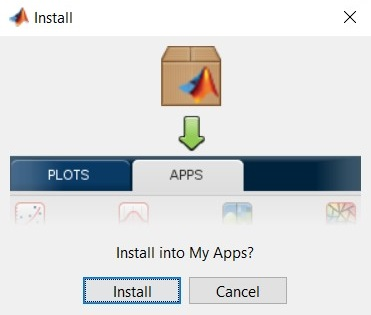
\includegraphics[width=0.5\textwidth]{InstallIntoMyApps.jpg}
\label{fig:installpopup}
\end{figure}
\end{enumerate}

\section{Opening the Applet}

\begin{enumerate}[label = Step \arabic*.]

\item Open MATLAB. \\
\item Left-click on the "APPS" tab in the top left corner of the MATLAB environment
\begin{figure}[H]
\centering
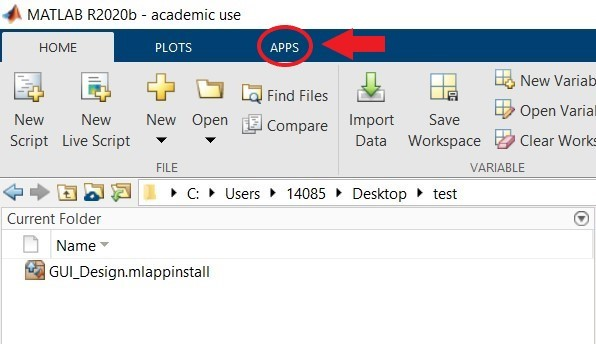
\includegraphics[width=0.5\textwidth]{FindingApps.jpg}
\label{fig:appstablocation}
\end{figure} 

\item Left-click on the dropdown menu in the APPS bar.
\begin{figure}[H]
\centering
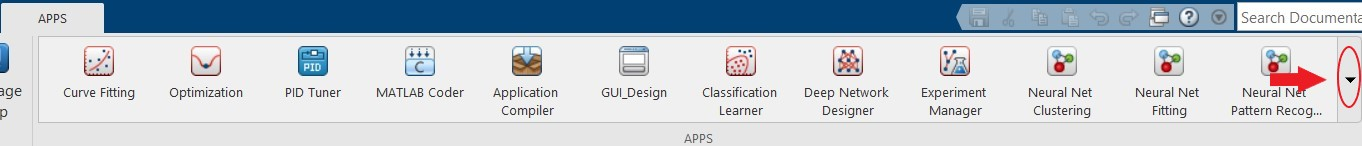
\includegraphics[width=\textwidth]{APPSDropDown.jpg}
\label{fig:appsdropdown}
\end{figure}

\item From the dropdown menu, left-click GUI\_Design from the "MY APPS" section.
\begin{figure}[H]
\centering
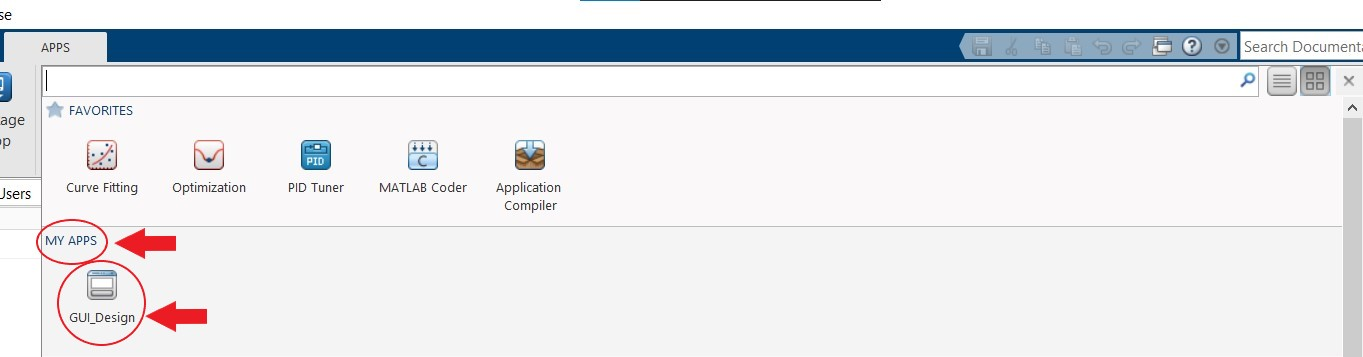
\includegraphics[width=0.5\textwidth]{MyAppsSection.jpg}
\label{fig:myappssection}
\end{figure}

\end{enumerate}

\section{Using the Applet}

\subsection{Uploading a Video}

\begin{enumerate}[label = Step \arabic*.]

\item Left-click on the "Upload Video" button. 
\begin{figure}[H]
\centering
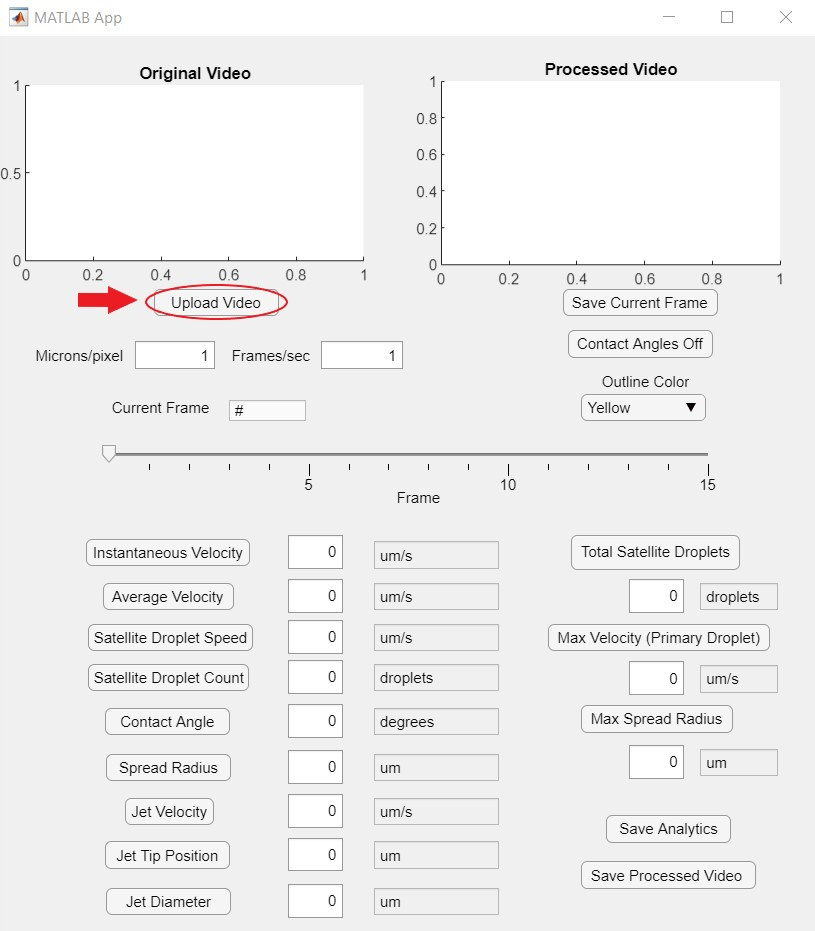
\includegraphics[width=0.5\textwidth]{appletbeforeupload.jpg}
\label{fig:uploadvideobutton}
\end{figure}

\item Select the video you would like to upload from the File Explorer window. Select "Open" to open that video file in the applet. The applet will open a secondary window for floor selection. You can either use the interactive floor finding or input the floor height in pixels and the floor angle. \\

\end{enumerate}

\subsubsection{Interactive Floor Finding}
\begin{enumerate}[label = Step \arabic*.]

\item Left-click the "Start Interactive Floor Find" button.
\begin{figure}[H]
\centering
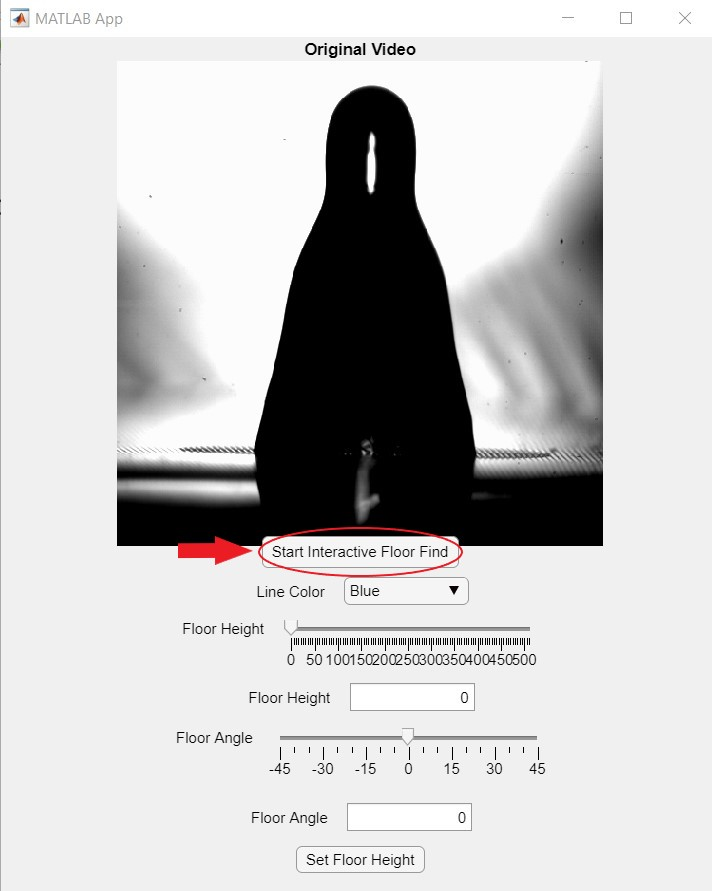
\includegraphics[width=0.5\textwidth]{SecondaryAppletFloorFindButton.jpg}
\label{fig:interactivefloorfindbutton}
\end{figure}

\item An instructional message will appear, informing the user that they can now draw a line at the floor on the video frame. Press the "OK" button to proceed with the interactive floor finding.
\begin{figure}[H]
\centering
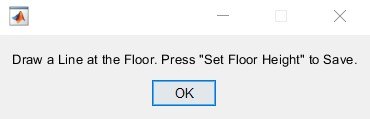
\includegraphics[width=0.5\textwidth]{DrawALineMsg.jpg}
\label{fig:drawalinemsg}
\end{figure}

\item Left-click and drag on the image to draw a line for the floor. To move this line, left-click and drag either blue dot at the ends of the line. Use the "Zoom-In" feature in the upper right-hand corner of the image to get a better look at where the floor line is located on the image. Continue manipulating the line by moving the blue dots until the interactive floor line matches the line of the floor in the original image. Press "Set Floor Height" Button once the interactive line is aligned.

\begin{figure}[H]
\centering
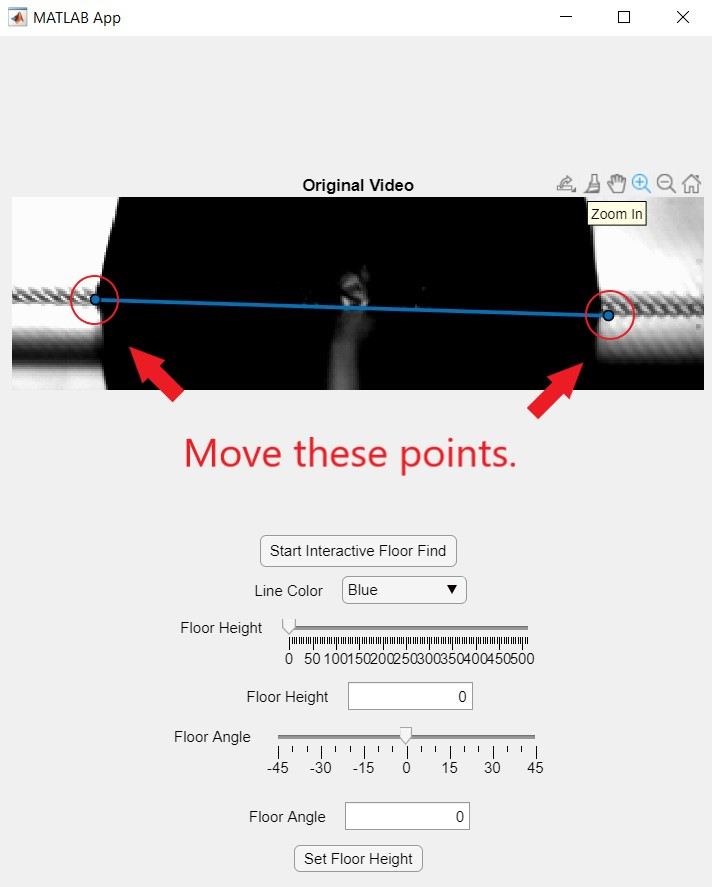
\includegraphics[width=0.5\textwidth]{InteractiveFloorLine.jpg}
\label{fig:interactiveline}
\end{figure}

\subsubsection{Manual Floor Height and Angle Entry}
During the manual floor height and angle entry process, if the line is difficult to see, the user can select a different line option from the "Line Color" dropdown menu. This feature is ONLY available for the line printed by manual floor height and angle entry.


\item Move the slider next to "Floor Height" or manually enter floor height value into the textbox below to set a floor height. Note: "Floor Height" is measured in pixels, counting the number of pixels from the top of the image to the centermost pixel of the floor line.
\begin{figure}[H]
\centering
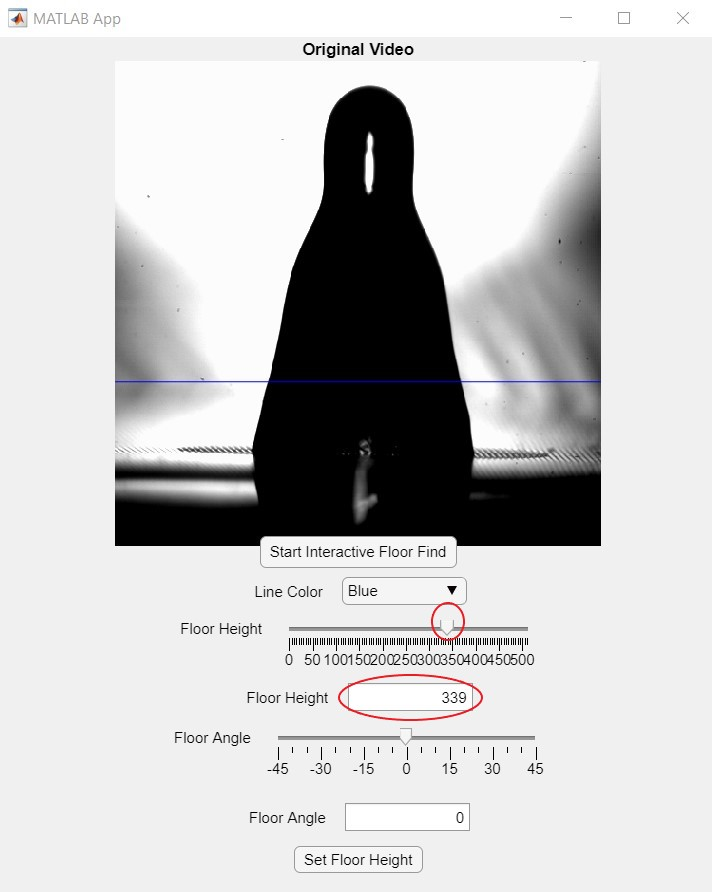
\includegraphics[width=0.5\textwidth]{ManualFloorHeight.jpg}
\label{fig:manualfloorheightslct}
\end{figure}

\item Move the slider next to "Floor Angle" or manually enter floor angle value into the textbox below to set a floor angle. 
\begin{figure}[H]
\centering
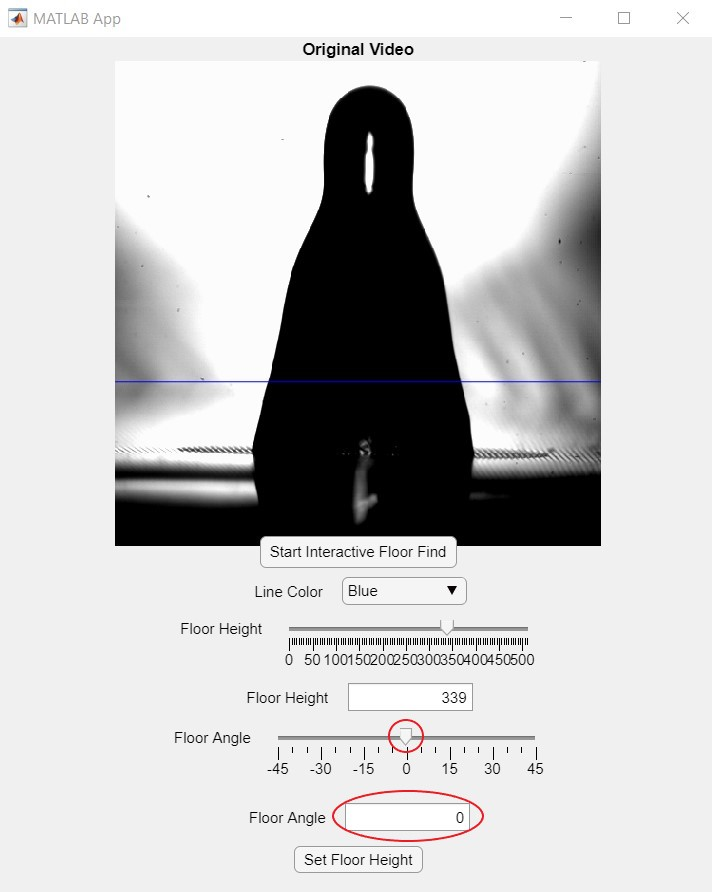
\includegraphics[width=0.5\textwidth]{ManualFloorAngle.jpg}
\label{fig:manualfloorangleslct}
\end{figure}

\item Once both floor height and floor angle are at the correct values, left-click the "Set Floor Height" button to input the floor values.

\item Once the floor height and angle has been set, the applet will process the entire video, then display the processed video. Please note, this process takes a lot of computation and will take time, especially on computers with limited processing power. 
\begin{figure}[H]
\centering
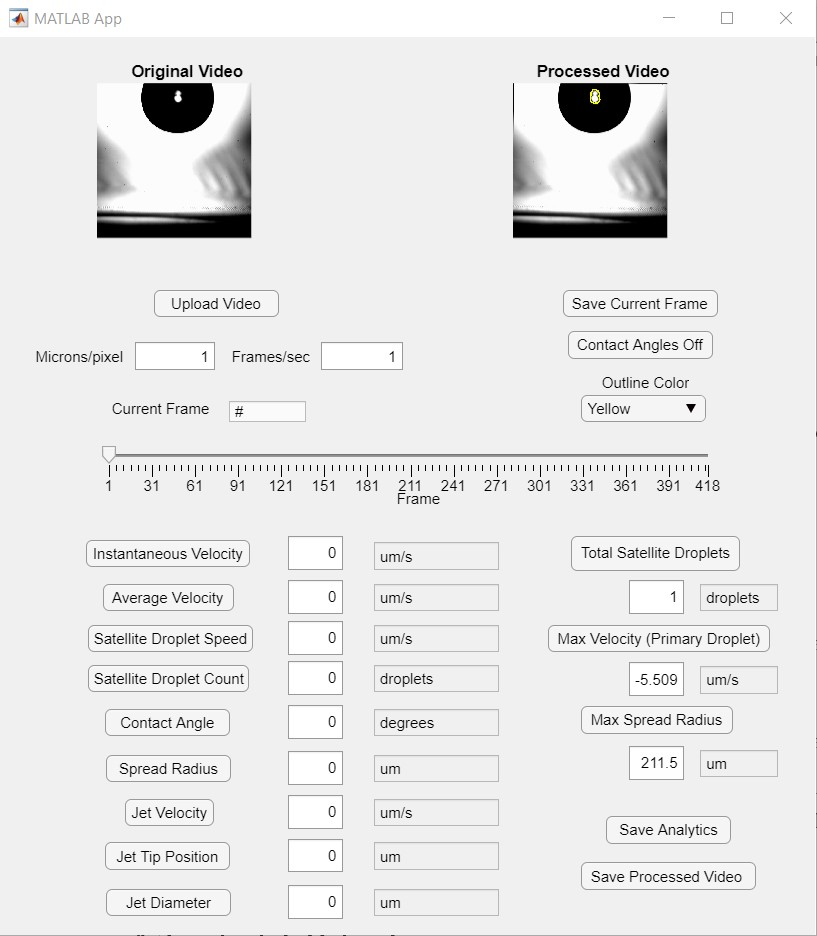
\includegraphics[width=0.5\textwidth]{FirstProcessedVideoImage.jpg}
\label{fig:rightafterfloorfind}
\end{figure}
\end{enumerate}

\subsection{Applet Features}












\chapter{System Functions}
In this chapter each of the image processing and droplet analysis functions are described. A paragraph of the system theory is given and describes the overall operation of the function and the variables in it. A fault isolation section is also provided which gives solutions and fixes to possible issues that may arise. 

\section{borders}
\subsection{Theory and Description}
The borders function is the second video processing function applied to the source video. 

\subsection{Fault Isolation}
\lipsum[4]



\section{calculateVelocity}
\subsection{Theory and Description}
\lipsum[4]

\subsection{Fault Isolation}
\lipsum[4]



\section{contactAngles}
\subsection{Theory and Description}
\lipsum[4]

\subsection{Fault Isolation}
\lipsum[4]



\section{convertSource}
\subsection{Theory and Description}
\lipsum[4]

\subsection{Fault Isolation}
\lipsum[4]




\section{drawContactAngles}
\subsection{Theory and Description}
\lipsum[4]

\subsection{Fault Isolation}
\lipsum[4]




\section{fallVelocity}
\subsection{Theory and Description}
\lipsum[4]

\subsection{Fault Isolation}
\lipsum[4]




\section{floorremove}
\subsection{Theory and Description}
\lipsum[4]

\subsection{Fault Isolation}
\lipsum[4]




\section{frame2file}
\subsection{Theory and Description}
\lipsum[4]

\subsection{Fault Isolation}
\lipsum[4]




\section{jetVelocity}
\subsection{Theory and Description}
\lipsum[4]

\subsection{Fault Isolation}
\lipsum[4]




\section{maskOverlay}
\subsection{Theory and Description}
\lipsum[4]

\subsection{Fault Isolation}
\lipsum[4]




\section{maxSpread}


\subsection{Theory and Description}
The droplet radius spreading feature determines the radius of the droplet on the left and right side, and provide the maximum radius the droplet in the video. Radii is only calculated after the droplet has made contact with the floor.
\newline
\newline
This function begins by determining the number of frames in dataset ('d').  Once the length is determined, it finds the last frame that is completely black (no droplet appears) and saves it as 'frame'. A new dataset is created from the original, this time eliminating the frames without any droplet. 

\subsection{Fault Isolation}




\section{outlineMask}\subsection{Theory and Description}
\lipsum[4]

\subsection{Fault Isolation}
\lipsum[4]




\section{outlines}
\subsection{Theory and Description}
\lipsum[4]

\subsection{Fault Isolation}
\lipsum[4]




\section{removePartialDroplet}
\subsection{Theory and Description}
\lipsum[4]

\subsection{Fault Isolation}
\lipsum[4]




\section{video2frame}
\subsection{Theory and Description}
\lipsum[4]

\subsection{Fault Isolation}
\lipsum[4]




































\chapter{Other Nonfunctional Requirements}

\section{Performance Requirements}
\par Matlab requirements are needed. Found at \url{https://www.mathworks.com/support/requirements/matlab-system-requirements.html}

\section{Safety Requirements}
\lipsum[4]

\section{Security Requirements}
\lipsum[4]

\section{Software Quality Attributes}
\lipsum[4]

\section{Business Rules}
\lipsum[4]









\chapter{Other Requirements}



\chapter{Appendix A: Glossary}

Dataset: Any video file that has been uploaded to MATLAB.\newline
Floor: (Variable) The horizontal reference in which the droplet impacts and begins spreading. \newline




\chapter{Appendix B: Analysis Models}




\chapter{Appendix C: TBD}






\end{document}
